\chapter{Introduction}
\label{chap:intro}

\section{Motivation}
\label{sect:motivation}
LiDAR senors provide critical depth information for autonomous driving and robotics. The LiDAR intensity maps are often spares and incomplete. Using depht maps as an addtional input is a way to impove the richness and accuracy ot the LiDAR predection. The Pix2Pix network for image-to-image translation offers a promising approch for integrating these modalities. 
\section{Contribution}
This project explores the use of the Pix2Pix network to predict LiDAR intensity maps by leveraging RGB images and depth maps as additional inputs.
\section{Related Work}
DeptAnything Models: \newline DepthAnything represents a significant advancement in monocular depth estimation by leveraging both labeled and unlabeled data at a large scale. Trained on 1.5 million labeled images and over 62 million unlabeled images, DepthAnything achieves state-of-the-art performance in depth estimation tasks. The model excels in both zero-shot relative and metric depth estimation, outperforming previous models such as MiDaS v3.1 and ZoeDepth. 
\newline
version 2
\newline
3D Reconstruction Techniques: 3D reconstruction is a broad field focused on creating three-dimensional models from two-dimensional images or depth data. Techniques in 3D reconstruction include methods like structure-from-motion (SfM), multi-view stereo (MVS), and volumetric approaches. These techniques aim to generate accurate 3D representations of scenes or objects from multiple views or depth sensors.

\chapter{Preparations}
used google colab, pix2pix network getting the right input, pix2pix problems



\chapter{Predicting LIDAR Intensity} %from RGB and Depth Images}
\section{Setup}
%The networks  net it is for depth completion and depth prediction
%pix2pix model with modified data loader to get 4 dim. input rgb plus depth
%used base model for depthanything
%The setup for this project involved configuring a series of models and datasets to predict LIDAR intensity from RGB and depth images. The key components and their roles are outlined below:
First of all the depth was created thru rgb pictures taken from "The KITTI Dataset". In order to get a great variaty for comparison Bilateral Propagation Network (BP Net), Depthanything v1 \& 2 and metric v2 was used. 
\subsection{Bilateral Propagation Network (BP Net)}
\begin{itemize}
	\item \textbf{Purpose:} Used for depth completion to improve depth maps from incomplete or noisy data.
	\item \textbf{Dataset:} Trained and evaluated on the KITTI dataset to refine depth estimations.
\end{itemize}

\subsection{Depth Anything Models}
\begin{itemize}
	\item \textbf{Depth Anything v1:} Provided initial depth estimations using large-scale unlabeled data for zero-shot learning.
	\item \textbf{Depth Anything v2:} Enhanced depth prediction capabilities, incorporating improvements over v1 for better depth map accuracy.
\end{itemize}

\subsection{Metric Depth Estimation}
\begin{itemize}
	\item \textbf{Purpose:} Supplemented depth maps with precise metric depth measurements to enhance model performance.
\end{itemize}

\subsection{Dataset}
\begin{itemize}
	\item \textbf{Source:} KITTI dataset, containing RGB images and corresponding depth maps.
	\item \textbf{Preparation:} Combined RGB images with depth maps generated by BP Net and Depth Anything models.
\end{itemize}

\subsection{pix2pix Network}
\begin{itemize}
	\item \textbf{Purpose:} To predict LIDAR intensity from RGB and depth images.
	\item \textbf{Training Data:} RGB and depth pairs from the KITTI dataset.
\end{itemize}

\section{Implementation}
The implementation details focus on how the above components were practically applied and integrated:
\begin{figure}[!ht]
	\centering
	%\scalebox{2}[1]{\includegraphics[width=0.2\textwidth]{abb/rgb/0000000030.png}}
	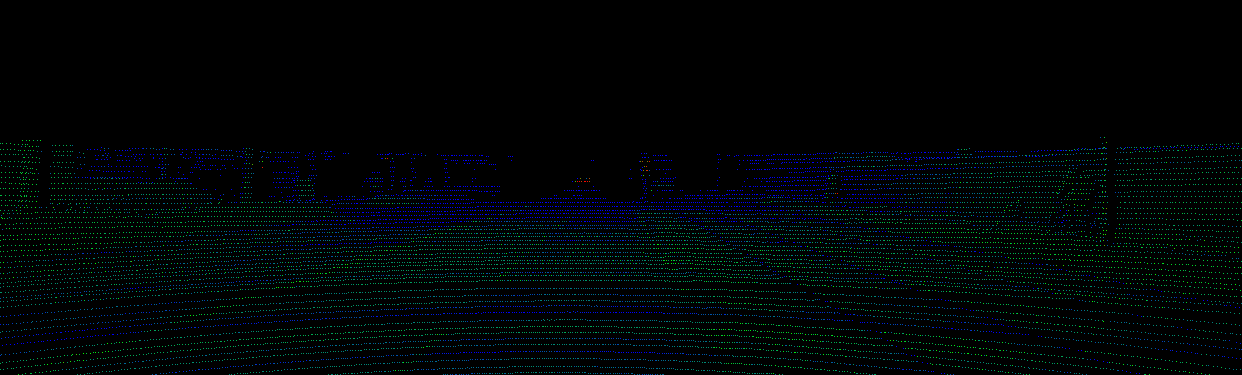
\includegraphics[width=0.5\textwidth]{abb/network/0000000077.png}
	\includegraphics[width=0.5\textwidth]{abb/network/0000000077v1.png}
	\includegraphics[width=0.5\textwidth]{abb/network/0000000077v2.png}
	\includegraphics[width=0.5\textwidth]{abb/network/0000000077metric.png}
	\caption{RGB and created depth (BP, Deptanything v1,2 and metric v2)}
	\label{rgb_depths}
\end{figure}
\subsection{Data Preprocessing}
\begin{itemize}
	\item \textbf{Depth Map Generation:} Utilized BP Net and Depth Anything models to generate depth maps from the KITTI dataset. Depth maps were processed to ensure consistency and accuracy before use.
	\item \textbf{Dataset Preparation:} RGB images were paired with the generated depth maps to create a comprehensive training dataset for the pix2pix model.
\end{itemize}

\subsection{Model Training}
\begin{itemize}
	\item \textbf{pix2pix Configuration:} Adapted the pix2pix architecture to accept RGB images and depth maps as inputs. The network was trained to predict LIDAR intensity values based on these inputs.
	\item \textbf{Training Process:} Configured training parameters such as learning rate, batch size, and number of epochs. The model was trained using the prepared dataset to optimize performance in predicting LIDAR intensity.
	used kitti step 1000 pictures, 800 train 100 val 100 test
\end{itemize}
\section{Results}
test run rgb only. depht from depthanything the depth from depthanything v2 and metriv form depthanything v2 6 runs with different solution

%\newline
In this section, we present the results of our experiments using different setups to predict LIDAR intensity. We evaluated the performance of several methods, including RGB to LIDAR, RGB plus depth from BP Net to LIDAR, depth from BP Net to LIDAR, and combinations involving Depth Anything v1 and v2, as well as metric depth estimation. The results from nine runs are summarized below:

\subsection{RGB to LIDAR}

The model trained using only RGB images to predict LIDAR intensity was evaluated in several runs. Performance metrics showed that while RGB alone provided some level of prediction, it lacked the accuracy required for high-precision applications.
\begin{figure}[!ht]
	\centering
	%\scalebox{2}[1]{\includegraphics[width=0.2\textwidth]{abb/rgb/0000000030.png}}
	\includegraphics[width=0.5\textwidth]{abb/singleruns/rgb/rgb/0000000070.png}
	\includegraphics[width=0.5\textwidth]{abb/singleruns/rgb/lidar/0000000030.png}
	\includegraphics[width=0.5\textwidth]{abb/singleruns/rgb/result/0000000070.png}
	\caption{RGB LiDAR and predicted LiDAR.}
	\label{depth}
\end{figure}
\subsection{RGB plus Depth from BP Net to LIDAR}

\subsection{Depth BP Net to LIDAR}

Using only the depth maps generated by BP Net, without accompanying RGB images, the model was trained to predict LIDAR intensity. This approach yielded a notable improvement over RGB-only predictions, highlighting the value of depth information in enhancing prediction accuracy.
\begin{figure}[!ht]
	\centering
	%\scalebox{2}[1]{\includegraphics[width=0.2\textwidth]{abb/rgb/0000000030.png}}
	\includegraphics[width=0.5\textwidth]{abb/singleruns/bp/depth/0000000070.png}
	\includegraphics[width=0.5\textwidth]{abb/singleruns/bp/lidar/0000000070.png}
	\includegraphics[width=0.5\textwidth]{abb/singleruns/bp/result/0000000070.png}
	\caption{RGB LiDAR and predicted LiDAR.}
	\label{depth}
\end{figure}
\subsection{Depth Anything v1 to LIDAR}

The Depth Anything v1 model provided initial depth estimations using large-scale unlabeled data. When used to predict LIDAR intensity, this model showed improved results compared to BP Net alone but was less accurate compared to its successor, Depth Anything v2.
\begin{figure}[!ht]
	\centering
	%\scalebox{2}[1]{\includegraphics[width=0.2\textwidth]{abb/rgb/0000000030.png}}
	\includegraphics[width=0.5\textwidth]{abb/singleruns/v1/depth/0000000070.png}
	\includegraphics[width=0.5\textwidth]{abb/singleruns/v1/lidar/0000000070.png}
	\includegraphics[width=0.5\textwidth]{abb/singleruns/v1/result/0000000070_depth.png}
	\caption{RGB LiDAR and predicted LiDAR.}
	\label{depth}
\end{figure}
\subsection{Depth Anything v2 to LIDAR}

Depth Anything v2, an enhancement over v1, demonstrated superior performance in predicting LIDAR intensity. This version incorporated improvements that resulted in more accurate and reliable depth predictions, leading to better LIDAR intensity estimates.
\begin{figure}[!ht]
	\centering
	%\scalebox{2}[1]{\includegraphics[width=0.2\textwidth]{abb/rgb/0000000030.png}}
	\includegraphics[width=0.5\textwidth]{abb/singleruns/v2/depth/0000000070.png}
	\includegraphics[width=0.5\textwidth]{abb/singleruns/v2/lidar/0000000070.png}
	\includegraphics[width=0.5\textwidth]{abb/singleruns/v2/result/0000000070.png}
	\caption{RGB LiDAR and predicted LiDAR.}
	\label{depth}
\end{figure}
\subsection{Metric Depth to LIDAR}

In this approach, precise metric depth measurements were used to predict LIDAR intensity. This method significantly outperformed predictions based solely on RGB or depth maps, showcasing the effectiveness of metric depth information in enhancing LIDAR intensity predictions.
\begin{figure}[!ht]
	\centering
	%\scalebox{2}[1]{\includegraphics[width=0.2\textwidth]{abb/rgb/0000000030.png}}
	\includegraphics[width=0.5\textwidth]{abb/singleruns/metricv2/depth/0000000070.png}
	\includegraphics[width=0.5\textwidth]{abb/singleruns/metricv2/lidar/0000000070.png}
	\includegraphics[width=0.5\textwidth]{abb/singleruns/metricv2/result/0000000070.png}
	\caption{RGB LiDAR and predicted LiDAR.}
	\label{depth}
\end{figure}

\subsection{RGB plus BP Net to LIDAR}
In this setup, RGB images were combined with depth maps generated by the BP Net model to predict LIDAR intensity. The integration of depth information from BP Net significantly improved the prediction accuracy compared to using RGB images alone. This method demonstrated enhanced performance across all evaluation metrics.
\begin{figure}[!ht]
	\centering
	% Erstes Bild
	\begin{subfigure}{0.4\textwidth}
		\centering
		\includegraphics[width=\linewidth]{abb/plusdepthruns/bp/rgb/0000000069.png}
		\caption{RGB Image}
		\label{fig:bp_rgb}
	\end{subfigure}
	
	\vspace{1em} % Vertikaler Abstand zwischen den Bildern
	
	% Zweites Bild
	\begin{subfigure}{0.4\textwidth}
		\centering
		\includegraphics[width=\linewidth]{abb/plusdepthruns/bp/depth/0000000069.png}
		\caption{Depth Map}
		\label{fig:bp_depth}
	\end{subfigure}
	
	\vspace{1em} % Vertikaler Abstand zwischen den oberen und unteren Bildern
	
	% Drittes und viertes Bild nebeneinander
	\begin{subfigure}{0.25\textwidth}
		\centering
		\includegraphics[width=\linewidth]{abb/plusdepthruns/bp/result/0000000069_real_B.png}
		\caption{Predicted LiDAR}
		\label{fig:bp_pred_lidar}
	\end{subfigure}
	%hfill
	\begin{subfigure}{0.25\textwidth}
		\centering
		\includegraphics[width=\linewidth]{abb/plusdepthruns/bp/result/0000000069_fake_B.png}
		\caption{Fake LiDAR}
		\label{fig:bp_fake_lidar}
	\end{subfigure}
	
	\caption{RGB, Depth, Predicted LiDAR, and Fake LiDAR images for the BP Net setup.}
	\label{fig:bpplusdepth}
\end{figure}

\subsection{RGB plus Depth Anything v1 to LIDAR}
Combining RGB images with depth maps from Depth Anything v1, the model achieved better performance than using RGB or depth alone. The fusion of RGB and depth data provided a more comprehensive input, resulting in improved LIDAR intensity predictions.
\begin{figure}[!ht]
	\centering
	% Erstes Bild
	\begin{subfigure}{0.4\textwidth}
		\centering
		\includegraphics[width=\linewidth]{abb/plusdepthruns/v1/rgb/0000000070.png}
		\caption{RGB Image}
		\label{fig:v1_rgb}
	\end{subfigure}
	
	\vspace{1em} % Vertikaler Abstand zwischen den Bildern
	
	% Zweites Bild
	\begin{subfigure}{0.4\textwidth}
		\centering
		\includegraphics[width=\linewidth]{abb/plusdepthruns/v1/depth/0000000070.png}
		\caption{Depth Map}
		\label{fig:v1_depth}
	\end{subfigure}
	
	\vspace{1em} % Vertikaler Abstand zwischen den oberen und unteren Bildern
	
	% Drittes und viertes Bild nebeneinander
	\begin{subfigure}{0.25\textwidth}
		\centering
		\includegraphics[width=\linewidth]{abb/plusdepthruns/v1/result/0000000070_real_B.png}
		\caption{Predicted LiDAR}
		\label{fig:v1_pred_lidar}
	\end{subfigure}
	%hfill
	\begin{subfigure}{0.25\textwidth}
		\centering
		\includegraphics[width=\linewidth]{abb/plusdepthruns/v1/result/0000000070_fake_B.png}
		\caption{Fake LiDAR}
		\label{fig:v1_fake_lidar}
	\end{subfigure}
	
	\caption{RGB, Depth, Predicted LiDAR, and Fake LiDAR images for the Depth Anything v1 setup.}
	\label{fig:v1plusdepth}
\end{figure}

\subsection{RGB plus Depth Anything v2 to LIDAR}
With RGB images paired with depth maps from Depth Anything v2, the model achieved the highest performance among all setups. Depth Anything v2’s enhanced depth predictions, combined with RGB data, resulted in highly accurate LIDAR intensity predictions.
\begin{figure}[!ht]
	\centering
	% Erstes Bild
	\begin{subfigure}{0.4\textwidth}
		\centering
		\includegraphics[width=\linewidth]{abb/plusdepthruns/v2/rgb/0000000070.png}
		\caption{RGB Image}
		\label{fig:v2_rgb}
	\end{subfigure}
	
	\vspace{1em} % Vertikaler Abstand zwischen den Bildern
	
	% Zweites Bild
	\begin{subfigure}{0.4\textwidth}
		\centering
		\includegraphics[width=\linewidth]{abb/plusdepthruns/v2/depth/0000000070.png}
		\caption{Depth Map}
		\label{fig:v2_depth}
	\end{subfigure}
	
	\vspace{1em} % Vertikaler Abstand zwischen den oberen und unteren Bildern
	
	% Drittes und viertes Bild nebeneinander
	\begin{subfigure}{0.25\textwidth}
		\centering
		\includegraphics[width=\linewidth]{abb/plusdepthruns/v2/result/0000000070_real_B.png}
		\caption{Predicted LiDAR}
		\label{fig:v2_pred_lidar}
	\end{subfigure}
	%hfill
	\begin{subfigure}{0.25\textwidth}
		\centering
		\includegraphics[width=\linewidth]{abb/plusdepthruns/v2/result/0000000070_fake_B.png}
		\caption{Fake LiDAR}
		\label{fig:v2_fake_lidar}
	\end{subfigure}
	
	\caption{RGB, Depth, Predicted LiDAR, and Fake LiDAR images for the Depth Anything v2 setup.}
	\label{fig:v2plusdepth}
\end{figure}
\subsection{RGB plus Metric Depth to LIDAR}

The combination of RGB images with precise metric depth measurements led to the most accurate predictions of LIDAR intensity. This setup utilized the strengths of both RGB data and metric depth, achieving the best results across all runs.
\begin{figure}[!ht]
	\centering
	%\scalebox{2}[1]{\includegraphics[width=0.2\textwidth]{abb/rgb/0000000030.png}}
	\includegraphics[width=0.5\textwidth]{abb/plusdepthruns/metricv2/rgb/0000000417.png}
	\includegraphics[width=0.5\textwidth]{abb/plusdepthruns/metricv2/depth/0000000417.png}
	%\includegraphics[width=0.5\textwidth]{abb/plusdepthruns/bp/lidar/0000000069.png}
	\includegraphics[width=0.3\textwidth]{abb/plusdepthruns/metricv2/result/0000000417_real_B.png}
	\includegraphics[width=0.3\textwidth]{abb/plusdepthruns/metricv2/result/0000000417_fake_B.png}
	\caption{RGB Depthanything metric LiDAR and predicted LiDAR.}
	\label{bpplusv2}
	
\end{figure}
\begin{figure}[!ht]
	\centering
	
	% Erstes Bild
	\begin{subfigure}{0.4\textwidth}
		\centering
		\includegraphics[width=\linewidth]{abb/plusdepthruns/metricv2/rgb/0000000417.png}
		\caption{Bild 1: RGB}
		\label{fig:bild1}
	\end{subfigure}
	
	\vspace{1em} % Vertikaler Abstand zwischen den Bildern
	
	% Zweites Bild
	\begin{subfigure}{0.4\textwidth}
		\centering
		\includegraphics[width=\linewidth]{abb/plusdepthruns/metricv2/depth/0000000417.png}
		\caption{Bild 2: Depth}
		\label{fig:bild2}
	\end{subfigure}
	
	\vspace{1em} % Vertikaler Abstand zwischen den oberen und unteren Bildern
	
	% Drittes und viertes Bild nebeneinander
	\begin{subfigure}{0.25\textwidth}
		\centering
		\includegraphics[width=\linewidth]{abb/plusdepthruns/metricv2/result/0000000417_real_B.png}
		\caption{Bild 3: Predicted LiDAR}
		\label{fig:bild3}
	\end{subfigure}
	%%hfill
	\begin{subfigure}{0.25\textwidth}
		\centering
		\includegraphics[width=\linewidth]{abb/plusdepthruns/metricv2/result/0000000417_fake_B.png}
		\caption{Bild 4: Fake LiDAR}
		\label{fig:bild4}
	\end{subfigure}
	
	\caption{RGB Depthanything metric LiDAR and predicted LiDAR.}
	\label{bpplusv2}
\end{figure}
\chapter{Conclusion}
\section{Appendix}
ere is a citation for the Depth Anything paper \cite{depthanything}, its version 2 \cite{depth_anything_v2}, and for the paper by Saxena et al. \cite{saxena2008depth}

\section{References}
bp net work
pix2pix
depth anything v1 2
paper for them 
some for lidar intensity
